\documentclass{llncs}

\usepackage[ruled,linesnumbered,vlined,boxed]{algorithm2e}
\usepackage{graphicx}
\usepackage{subfigure}
\usepackage[cmex10]{amsmath}
\usepackage{amssymb, latexsym}
\usepackage{pst-all}
\usepackage{url}

\usepackage{xcolor}
\usepackage{tikz}
\usetikzlibrary{scopes}

\newcommand{\keywords}[1]{\par\addvspace\baselineskip
\noindent\keywordname\enspace\ignorespaces#1}

\begin{document}

\title{A Topology Control Algorithm for Interference and Energy Efficiency in Wireless Sensor Networks}

\author{Hugo Braga\thanks{The work of this author was partially supported by CAPES (Coordenaç\c{c}\~ao de Aperfei\c{c}oamento
de Pessoal de N\'ivel Superior), Brazil} \and Fl\'avio Assis}
\institute{
LaSiD - Distributed Systems Laboratory\\
DCC - Department of Computer Science\\
PPGM - Graduate Program on Mechatronics \\
UFBA - Federal University of Bahia\\
Salvador, Bahia, Brazil\\
{\{hugobraga,}
{fassis\}}@ufba.br
}

\maketitle

\newtheorem{mydef}{Definition}

\begin{abstract}
Topology control is one of the main techniques that can be used to decrease energy expenditure and/or interference in wireless sensor networks. 
Less attention, however, has been devoted to algorithms that address energy and interference efficiency together. 
In this paper, we describe a localized topology control algorithm called TCO which is very efficient in terms of interference while minimizing energy efficiency. 
In order to evaluate TCO in terms of interference and compare it with other algorithms,
we defined a new metric called PICS (Path Interference Cost based on Sender) Spanning Factor. According to this metric, in our experiments TCO outperformed all related localized topology control 
algorithms and its performance was extremely close to the performance of a centralized algorithm which is optimal according to the PICS spanning factor
(a variation of ATASP based on PICS).
\keywords{Wireless Sensor Networks, Topology Control, Overhearing, Interference, Energy Efficiency.}
\end{abstract}

\section{Introduction}

A Wireless Sensor Network (WSN) is a special type of wireless network whose nodes have limited resources in terms of energy supply (they are usually battery-operated), 
computation power and memory. Conserving energy is thus a key issue in the design of WSNs.
\textit{Topology control} is one of the main techniques used to conserve energy. The goal of topology control is to determine a transmission power 
to each node of the network with the purpose of maintaining some property (e.g. connectivity) over the resulting communication graph while reducing the energy consumed by the nodes and/or
the interference in the network \cite{Santi05a}. 

Although optimizing energy efficiency and interference are at the core of topology control, most work does not consider these goals together.
Algorithms for topology control initially focused on energy efficiency. Interference was only considered implicitly, assuming that reducing the number
of neighbors of nodes resulted in low interference. In \cite{burkhart2004}, however, it was shown that low node degree does not imply low interference.
Therefore interference should be addressed explicitly. Since then different approaches
to topology control which attempt to optimize interference have been proposed. They are based on metrics that consider the \emph{number} of
nodes in specific areas affected by transmissions. These areas are dependent on the specific metric of interference
used.

In this paper, we describe a distributed localized algorithm based on a specific edge weight function which is efficient in terms of interference and energy expenditure.
This algorithm was presented in a previous work by one of the authors \cite{Assis09} 
as an algorithm for energy-efficiency which takes the cost of \emph{overhearing}
into consideration, i.e. the cost implied when nodes hear messages even if the messages are not intended for them. We will refer to this algorithm as \emph{TCO}
(from \emph{Topology Control considering Overhearing}).
In this paper we show that as the edge weight function used in TCO takes into consideration the transmission \emph{and} reception cost, including overhearing, it 
implicitly takes into consideration the number of nodes affected by a transmission. Thus, TCO optimizes energy \emph{and} interference at the same time. 

An important aspect of this work is that we deviate in the design of our algorithm from most existing work in two important ways. First, we take the cost of
overhearing into consideration (normally ignored in previous work on energy-efficient topology control). Second, we generate topologies that might be
asymmetric, i.e. on the final topology there might be an edge from a node $u$ to node $v$ but not from $v$ to $u$ (the final topology is, however,
strongly connected). We argue that the cost of overhearing is significant when considering currently used sensor nodes and MAC (\emph{Medium Access Control}) 
protocols and that, by taking this cost into consideration, we can generate topologies that are efficient both in terms of energy and interference. 
We argue additionally that generating asymmetric links might be useful in some situations and might even lead to energy conservation.

More specifically in this paper: 
(a) we argue that, unlike most previous work on topology control, it is important to take the cost of overhearing into consideration and it might be useful to generate topologies with
asymmetric links
(b) we show the impact of taking the cost of overhearing into consideration when optimizing energy and interference at the same time
(c) we propose a new metric for interference
(d) we present a specific edge weight function that incorporates energy and interference parameters and 
(e) we show a (distributed) localized topology control algorithm based on this function that is efficient in terms of energy (as shown in 
\cite{Assis09,Telemaco2009}) and interference. 
According to the defined interference metric, our algorithm outperformed existing algorithms described in the literature and, more importantly, although localized, 
it is extremely close to the performance of an optimal global solution (i.e. a solution based on the whole information about the network).

This paper is organized as follows.
Section \ref{sec-related-work} discusses related work. 
Section \ref{sec-support-tcoverhearing} presents our arguments in favor of considering the cost of overhearing and asymmetric links.
Section \ref{sec-system-model} describes the assumed system model.
Section \ref{sec-interference} introduces a new interference metric.
Section \ref{sec-algorithm} describes a topology control algorithm for optimizing energy efficiency and interference.
Section \ref{sec-evaluation} describes the results of experiments performed to evaluate the algorithm. 
Finally, Section \ref{sec-conclusion} concludes the paper.

\section{Related Work}
\label{sec-related-work}

To the best of our knowledge, \cite{burkhart2004} was the first work on topology control to address interference explicitly (in a traffic-independent way),
after pointing out that reducing node degree does not imply low interference.
The authors measured interference as the sum of the nodes in the range of two communicating nodes, a sender and a receiver. 
The idea is that these nodes are the ones which could hear a transmission from the sender and a corresponding
reply (such as an ACK message) from the receiver. 
This approach is classified as \mbox{\emph{link-based}} (according to the classification introduced in \cite{Li05}) because interference is based on the two endpoints of links,
and as \emph{sender-centric} (according to the classification introduced in \cite{fussen2005}) because interference
is considered from the perspective of the node sending a message.

Later, \cite{blough2005} argued that interference must be addressed considering multihop paths as messages
actually traverse such paths. An algorithm developed considering only one-hop paths does not necessarily
provide a good solution when multihop interference is considered. The authors thus proposed 
a multihop metric for interference, based on the link-based approach. 

In \cite{fussen2005} (and after that \cite{johansson2005}, \cite{moscibroda2005} and \cite{rickenbach2005}) the authors argued that interference
should be considered from the receiver perspective. According to these authors, a transmission can be affected
by the overall effect of different transmissions as perceived by the receiver. These authors thus introduced interference
metrics that are classified as \emph{receiver-centric}. The main idea is that the interference as perceived by
node $v$ is the number of all nodes $u$ such that $v$ is in the range of $u$'s transmissions. More recent work 
\cite{liu2008,Gao2008} addresses interference based on physical models (as opposed to graph-based
models, as used in previous work). Their notion of interference is naturally receiver-centric. 

% ?? adicionei uma frase abaixo: "We think ... "

However, as pointed out in \cite{damian2008}, adopting a sender-centric approach has the following benefits:
(a) it captures interference in certain scenarios better
and (b) it has been shown that a receiver-centric metric is limited by a constant factor of a sender-centric metric \cite{Burkhart03}\footnote{In \cite{Burkhart03} it was shown that the 
receiver-centric metric defined in \cite{rickenbach2005}, referred to as $I_{in}$, relates to the sender-centric metric defined in \cite{burkhart2004},
referred to as $I_{out}$, by the expression $I_{in} \le 5 . I_{out}$}, i.e. 
reducing the interference when a sender-centric metric is used implies that interference is reduced when a receiver-centric metric is used.
We think that a similar effect might also happen when the (sender-centric) metric defined is this paper is used.
Additionally, we argue that optimizing interference based on a receiver-centric approach is harder, because the level of interference to consider for a given
node $u$ depends on possible combinations of powers assigned to each of the nodes that might have $u$ in their ranges.

In fact, to the best of our knowledge, all algorithms that have been proposed to optimize interference
using a receiver-centric approach are centralized, i.e. they are based on global information about the communication graph 
\cite{fussen2005} \cite{moscibroda2005} \cite{rickenbach2005}
\cite{Wu2008} \cite{liu2008} and \cite{Gao2008}.
Some approaches to interference based on a sender-centric approach are also centralized \cite{burkhart2004} (LIFE and LISE) and \cite{blough2005} (ATASP). 
In particular, ATASP is an optimal algorithm considering multihop path interference (according to the PIC spanning factor - see Section \ref{sec-interference}). 
However, four localized sender-centric algorithms have been proposed:
LLISE \cite{burkhart2004}, API \cite{johansson2005}, I-LMST \cite{Li05} and I-RNG \cite{Li05}
(the authors in \cite{Li05} proposed an additional localized topology control algorithm that preserves spanning property - a more restrictive requirement which might
lead to worse solutions -, but we do not consider it here as 
we are not addressing spanning property). A distributed algorithm, SLISE \cite{damian2008}, has also been described, but it optimizes one-hop interference.

The algorithm that we describe in this paper, TCO, is sender-centric, localized and is based on multihop interference. It is therefore closely related to LLISE, API, I-LMST and \mbox{I-RNG}.
Additionally, according to the classification introduced in \cite{Li05}, it is based on an approach called \emph{node-based}, because interference is based on only one of the endpoints of links 
(in contrast to the \emph{link-based} approach). 
As presented in Section \ref{sec-evaluation}, our algorithm outperforms LIFE and all other localized algorithms related to ours. We compared our algorithm with LIFE instead of LLISE (both proposed in the same paper), because LIFE is a centralized algorithm 
which performs better than LLISE (according to the interference metric of their authors). 

TCO has been previously evaluated only in relation to energy efficiency \cite{Assis09,Telemaco2009}. 
The work described in this paper differs from \cite{Assis09,Telemaco2009} in that we address interference here.

\section{Overhearing Cost and Asymmetric Links}
\label{sec-support-tcoverhearing}

As mentioned before, TCO takes into consideration the cost of overhearing and the generated topology might contain asymmetric links. Most previous work on topology
control does not take the cost of overhearing into consideration. Additionally, the absence of asymmetric links in the generated topology is generally considered a good property. Thus,
our assumptions deviate from the assumptions commonly adopted in the literature. In this section, we argue why we think our assumptions are appropriate.

The cost of overhearing is one the major sources of energy expenditure due to communication in WSNs \cite{Misra2010}. Despite this, many MAC protocols are subject to overhearing.
All protocols that rely on \emph{low power listening} (or \emph{preamble sampling}) \cite{Polastre2004,Hoiydi2004,Buettner2006,Zhang2009,Ansari2010} suffer from overhearing,
basically due to their asynchronous nature. A node broadcasts a signal to every node in its vicinity to indicate its intention to transmit a message. Nodes in the vicinity might hear the
signal even if the message is not intended for them.
In particular, \mbox{B-MAC} \cite{Polastre2004}, a preamble sampling protocol, is the default MAC protocol for \emph{TinyOS} \cite{Buettner2006}, 
one of the most important operating systems for WSNs. Additionally, the MAC protocol specified in IEEE 802.15.4 \cite{Society2006}, a \emph{de facto} standard for the MAC and the physical layer for devices with low consumption, also suffers from overhearing. In IEEE 802.15.4, RTS/CTS signaling messages (which could be used to identify the sender and receiver of a transmission) 
are not used and nodes do not sleep during the so-called \emph{Contention Access Period} (each node needs to hear the transmissions to identify messages sent to it).

Furthermore, another argument in favor of considering overhearing is that the reception cost in current transceivers has tended to increase \cite{CC2530,RF230} and, for some specific
transceivers, it is higher than the transmission cost at maximum power (for example, for the Chipcon CC2420 transceiver \cite{CC2420}).

Regarding the presence of asymmetric links in the final topology, many topology control algorithms avoid it on the assumption that handling asymmetric links is difficult at the MAC
sublayer (for example, due to ACKs). However, we think that asymmetric links might be interesting in many specific situations and might even lead to energy conservation. 
In IEEE 802.15.4, for example, ACKs are optional (the need for the receiver to send an ACK is specified on a message basis) \cite{Society2006}. 
The need to acknowledge every message might be a source of unnecessary energy expenditure. Message broadcasting without
the need for guaranteeing reception at all nodes, such as in the case of beacons or specific messages (such as cryptographic keys as in \cite{deng02}) broadcast by the
base station to the whole network are also examples where asymmetric links can be used. Additionally, some authors have proposed eliminating ACKs in order to improve the 
performance of the network. For example, in \cite{Wu-X2006} the authors propose an energy efficient transport service (that includes both transport and MAC layers services), the PMC,  to transport events with a tradeoff between reliability and energy efficiency. PMC works over a Silent CSMA, which consists of a variant of CSMA/CA without ACKs. 
In \cite{ZhangY2008}, the authors propose a key establishment protocol for security services 
that explores unidirectional links. The advantage of this approach is that, instead of removing the unidirectional links as generally key establishment schemes do, 
the authors explore this type of link in order to improve connectivity and increase the network lifetime. 

\section{System Model}
\label{sec-system-model}

In this paper, a wireless sensor network consists of a set of $n$ static nodes. We model the behaviour
of each node by a \emph{process} associated with the node. Therefore we have $n$ processes, 
$p_1, p_2, ..., p_n$, one for each node. As there is a one-to-one correspondence between processes 
and nodes, we will use the terms \emph{process} and \emph{node} interchangeably.

We assume that each node can adjust its transmission power to any value between 0 and a certain 
maximum, referred to as $M_{power}$ (in the experiments described in this paper, however, each node transmits with one out of a
fixed number of power levels - see Section \ref{subsec-parameters}). The maximum power level is the same for
all nodes. Varying the transmission power of a node might change its set of neighbours. 
We assume that there is a path between any pair of nodes (processes) 
in the network, if all nodes transmit at $M_{power}$. 

Our energy model is based on the model presented in \cite{Heinzelman2002}. Energy is spent
by nodes during transmission, reception and during processing states. However, the energy spent 
during processing is neglected (we do not take the processing costs into consideration in this paper). The energy used to transmit is the energy spent to run the radio electronics
and the power amplifier. Both are dependent on hardware characteristics, such as the digital coding and 
modulation used. The energy used to run the power amplifier is also dependent on the distance 
between the transmitter and receiver and is computed according to a specific path loss model. 

Thus, the energy spent to transmit an $l$-bit message from process $p$ to process $q$, denoted 
$E_{Tx}(l, p, q)$, is given by:

\begin{equation}\label{eq-etx}
E_{Tx}(l, p, q) = l.E_{TxElec} + l.\epsilon.d^\alpha,
\end{equation}

where: $E_{TxElec}$ is the energy spent by the transmitter electronics; $d$ is the distance (in meter)
between $p$ and $q$; $\alpha$ is the path loss exponent (typically $2 \le \alpha < 6$); and $\epsilon$  is 
a parameter that is characteristic of the transceiver and the channel \cite{Rappaport1996}. 

The energy spent to receive an $l$-bit message, denoted $E_{Rx}(l)$, is given by:

\begin{equation}\label{eq-erx}
E_{Rx}(l) = l.E_{RxElec},
\end{equation}

where $RxElec$ is the energy spent to run the receiver electronics.

We assume that the nodes are distributed over a plane (i.e. the location
of each node is given by a pair of $x,y$-coordinates). Additionally, each process knows its current geographic location
(the nodes obtain this information from a positioning system, such as GPS, or by
other means, such as triangulation with some reference points in the network).

\section{A New Metric for Interference}
\label{sec-interference}

Different metrics have been proposed to quantify interference \cite{blough2005} \cite{Li05} \cite{burkhart2004} \cite{johansson2005} \cite{Moaveni-nejad05}. 
In most previous work interference is defined on a per link basis, instead of being based on paths. In \cite{blough2005}, the authors showed that topologies constructed based only on
links might not be efficient, when considering a path-based interference metric. However, in WSNs data generaly flow through multihop paths. Therefore, a metric based on multihop
paths seems more reasonable. In this section we define a new interference metric based on paths that differs from previous work as we consider asymmetric links.

In \cite{burkhart2004}, interference is defined based on the notion of link \textit{coverage}.
The coverage of a link $(u, v)$ represents the number of nodes that are inside the disks centered at $u$ and $v$ with radius $|u,v|$. The authors assume that links are bidirectional.
The coverage thus represents the set of nodes that are affected by a transmission over this link in both directions (to model that a transmission of a message from a node
$u$ to node $v$ is commonly followed by an acknowledgment message from $v$ to $u$). 
The authors in \cite{burkhart2004} additionally assume a simplistic model of circular coverage, i.e., they use the
UDG (Unit Disk Graph) model. 

% ?? alterei daqui ...

Due to the oversimplified nature of the UDG model, the authors in \cite{blough2005} introduced the \textit{Interference Number} (IN) of
an edge. The IN generalizes the concept of coverage. It is based on the fact that the area affected by a transmission might not be a perfect circle, rather an arbitrarily shaped area.
Let $p_{uv}$ be the minimum power that node $u$ needs to reach node $v$. 
The IN of an edge $(u,v)$, denoted $IN(u,v)$, is defined as $IN(u, v) = |covIN(u,v))|$ where:

\begin{equation}
\label{eq:ic_cov}
  covIN(u,v) = \lbrace w | w \in I(u,p_{uv}) \lor w \in I(v,p_{vu})\rbrace.
\end{equation}

In \eqref{eq:ic_cov}, for a node $z$, $I(z,p_{z})$ denotes the nodes affected (in some region) when node $z$ transmits with power $p_{z}$. There is no restriction on the geometry of the area
affected by a transmission.

The authors in \cite{Li05} present a notion of interference called \textit{Interference based on Sender}.
In \cite{Li05}, interference of a node $u$ represents the number of nodes affected when $u$ transmits with the minimum power needed to reach \emph{all}
its neighbours. 
We define \emph{Interference based on Sender} (IS) differently.  
We define $IS(u, v)$ as the set of nodes affected when $u$ transmits with power $p_{uv}$, i.e.: 

\begin{equation}
\label{eq:is_cov}
  IS(u, v)=|I(u, p_{uv})|. 
\end{equation}

% ?? ... ate aqui

Both the IN and the IS reflect the notion of interference presented in sender-centric approaches (see Section \ref{sec-related-work}).
In addition, IS reflects the node-based interference approach (see Section \ref{sec-related-work}).

In this paper, we propose a new interference metric based on paths, called \textit{Path Interference Cost based on Sender} (PICS). This metric is a variation
of the  \textit{Path Interference Cost} (PIC), proposed in \cite{blough2005}. 
Let $G(V,E)$ be a maximum power graph and $H(V,E')$ be a subgraph of $G$.
Let $p$ be a multihop path \mbox{$p$ = $\langle w_0,w_1, ..., w_{h-1}, w_{h} \rangle$} in $H$. We define the PICS for path
$p$ as:

\begin{equation}
\label{eq:new_pic}
  PICS(p) = \sum_{i = 0}^{h - 1}IS(w_i, w_{i+1}).
\end{equation}

The difference between our metric (PICS) and PIC \cite{blough2005} is that PIC is based on \textit{IN}, instead of on \textit{IS}, i.e. in the case of PICS 
the interference is based on node instead of being based on link.

Based on our PICS definition, we denote $mips^{G}_{uv}$ the \textit{minimum interference path based on sender} between a source node $u$ and a destination $v$ in a graph $G = (V,E)$,
i.e. a path $p$ between $u$ and $v$ for which PICS($p$) is the minimum. 

In order to quantify the amount of interference that a specific algorithm reduces in comparison to a maximum power graph, the authors in \cite{blough2005} introduced the
\textit{PIC Spanning Factor} ($\rho$). Adapting this concept to our definition of path interference cost, we define the \emph{PICS Spanning Factor} ($\sigma$) as follows.
Let $G = (V, E)$ be a maximum power communication graph, and let $H = (V, E')$ be a subgraph of G. The PICS spanning factor of $H$, $\sigma(H)$, is the average, 
over all possible source/destination pairs, of the ratio of the cost of a minimum interference path based on sender in $H$ to the cost of a minimum interference path based on sender in G. Formally,

\begin{equation}
\label{eq:new_spanning_factor}
  \sigma(H) = \frac{\sum_{\forall u,v \in V, u \not= v}\frac{PICS(mips^{H}_{uv})}{PICS(mips^{G}_{uv})}}{|\lbrace (u,v) | u,v \in V, u \not= v\rbrace |}.
\end{equation}

There are basically two differences between $\sigma$ and $\rho$: (a)  $\sigma$ is based on the notion of PICS instead of PIC and (b) $\sigma$ is based on an \textit{average} value instead of 
a \textit{maximum} value (of ratios). 
The former difference comes from the fact that we assume a node-based interference approach. The latter comes from the fact that we believe that 
the average value captures the notion of global interference in the network better. For example, for a specific pair of nodes $u$ and $v$, if the level of interference of the path between
them is high, the topology will be considered bad even if the interference levels for all other paths in the graph are good, if the maximum (interference value) is used. 
The average value circumvents this problem. 
The interference of a topology based on an average value is also used elsewhere \cite{johansson2005,Moaveni-nejad05,Banner2O08}.
  
\section{A Topology Control Algorithm that considers Overhearing}
\label{sec-algorithm}

The algorithm TCO determines the transmission power for each node by finding the node's \textit{reduced set of neighbours}. A node $q$ belongs to a node $p$'s reduced set of neighbors iff $q$ is one of $p$'s neighbours and the edge $(p, q)$ is not \emph{k-redundant}, considering $p$'s local information. 
An edge $(p, q)$ is k-redundant ($k \ge 2$) iff there is a path with length $k$
(i.e. with $k$ edges), such that sending a message from $p$ to $q$ along this path
has a lower cost (i.e. it results in less energy being spent) than sending the message directly from $p$ to $q$. 

All processes execute the same algorithm, shown in Figure \ref{alg:algoritmo}.
The algorithm has a directed graph $G^{2h}_p=(V^{2h}_p, E^{2h}_p)$ which represents the two-hop neighbourhood of process $p$ 
and the set $Pos_p$ as input. Let $G_{max}=(V, E_{max})$ be the graph generated when all nodes transmit at full power. $V^{2h}_p$ contains 
$p$, its neighbours (when transmitting at full power), and the neighbours of its neighbours (when transmitting at full power). Formally:
\begin{center}
$V_p^{2h}=\{p\} \cup \{ q  : q \in V$ $\land$ $(((p, q) \in E_{max})$ $\lor$ \linebreak 
$(\exists$ $r : r \in V \land (p, r) \in E_{max} \land (r, q) \in E_{max}))$\}  \\
and \\
$E_p^{2h}=\{ (p, q) : q \in V_p^{2h} \land (p, q) \in E_{max}\}$ $\cup$ \linebreak
\hspace*{\stretch{1}} $\{(r, s) : r \in V_p^{2h}$ $\land$ $s \in V_p^{2h}$ $\land$ 
	$(p, r) \in E_{max}$ $\land$ $(r, s) \in E_{max}\}$
\end{center}

\SetKwInOut{Input}{Input}
\SetKwInOut{Output}{Output}
\begin{algorithm}
\Input{$G_p^{2h}=(V_p^{2h}, E_p^{2h})$, $Pos_{p}$}
\Output{$myPower_p$}
\BlankLine
 $G_p^{min}(V_p^{min}, E_p^{min}) \gets $ \FuncSty{findMinCostPathsTree(} \ArgSty{p, $G_p^{2h}$, $Pos_p$} \FuncSty{)}\\
  $RNbrs_p \gets \lbrace q:q \in V_p^{min} \wedge (p,q) \in E_p^{min} \rbrace$ \\
  $highestSet_p \gets \{q : (q \in RNbrs_p)$ $\land$ 
           \hspace*{2.7cm} ($\nexists r : (r \in RNbrs_p) \land (power(p, r) > power(p, q)))\}$ \\
  $highest_p \gets$ any $q$ such that $q \in highestSet_p$ \\
%  $myPower_p \gets $ \FuncSty{power(}\ArgSty{$highest_p$}\FuncSty{)}
  $myPower_p \gets $ $power(p, highest_p)$
\caption{TCO (process $p$)} 
\label{alg:algoritmo}
\end{algorithm} 

The set $Pos_p$ is the set of 2-tuples $\langle q, \langle x_q, y_q \rangle \rangle$, where $x_q$ and $y_q$
are the Euclidian $x,y$-coordinates of process $q$. We do not specify a particular way for $p$ to obtain $G^{2h}_p$ and
$Pos_p$ as the focus of this paper is on the topology generated by the algorithm (they can be easily
obtained by the exchange of messages with topology information).

The algorithm is described for a generic process $p$.
First, $p$ calculates a tree of minimum cost paths from itself to each of its 2-hop neighbours (Fig. \ref{alg:algoritmo}, line 1). We represent an algorithm that finds this tree
by the procedure \verb|findMinCostPathsTree|. Any algorithm can be used to do this, however we impose as a requirement that,
if the edge $(p, q)$ is a minimum cost path between nodes $p$ and $q$, this edge is returned as the minimum cost path between
these nodes, instead of any other longer path with the same cost that might exist, i.e. the algorithm prefers one-edge paths instead of longer paths with the same
cost.

Subsequently, the $RNbrs_p$ set is determined (Fig. \ref{alg:algoritmo}, line 2). $RNbrs_p$ contains the set of nodes that are direct neighbours of $p$ in the computed
minimum cost paths tree. The set $highestSet_p$ contains the nodes $q$ in $RNbrs_p$ for which the edges $(p, q)$ have the highest cost (Fig. \ref{alg:algoritmo}, line 3).
We assume that there is a function $power(u, v)$ that determines the minimum power needed by node $u$ to reach node $v$.
As there may be more than one such node, $highest_p$ represents any of these nodes (Fig. \ref{alg:algoritmo}, line 4). Finally, the power assigned to $p$
is the minimum power needed by $p$ to reach $highest_p$ (Fig. \ref{alg:algoritmo}, line 5). 

Let $G_p^R = (V_p^R, E_p^R)$ be the directed graph that represents the relationship between
a process $p$ and its reduced set of neighbours, i.e. $V_p^R = \{p\} \cup RNbrs_p$
and $E_p^R = \{(p, q) : q \in RNbrs_p\}$. 

The resulting topology induced by the algorithm is the graph \linebreak \mbox{$G_{TCO}=(V, E_{TCO})$}, where $E_{TCO}$ is
defined as follows:
\begin{center}
\begin{displaymath}
E_{TCO} = \bigcup_{\forall p \in V}{E_p^R}
\end{displaymath}
\end{center}

TCO generates a topology that is strongly connected and that has the \linebreak \mbox{minimum-energy} property (see \cite{Assis09} for details).

\section{Evaluation}
\label{sec-evaluation}

TCO was analysed in terms of energy efficiency in \cite{Assis09,Telemaco2009}. In this section, we present the results of a series of experiments to show that  TCO also presents good performance in terms of interference. The main reason for this is that the edge weight function used in \mbox{TCO} takes into consideration energy
efficiency \emph{and} interference as it encompasses the number of nodes affected by transmissions (interference).

We first describe the parameters used in the experiments (Section \ref{subsec-parameters}). Then, we compare TCO with other topology control algorithms considering the interference metric defined in Section \ref{sec-interference} (Section \ref{subsec-evaluation_interference}).
 
\subsection{Experiment Parameters}
\label{subsec-parameters}

We built a specific Java program in order to perform the experiments. The communication and energy parameters used in the program were based on values extracted from the 
Chipcon CC2420 transceiver datasheet \cite{CC2420} since this transceiver is commonly used in wireless sensor networks. In particular, the program models the different transmission power levels
of the transceiver (a node transmits with one out of five power levels). 

% ?? no paragrafo abaixo, eu coloquei a unidade metro. Alem disso, coloquei TxElec e RxElec na sexta linha abaixo.

The maximum radio range of each node is approximately 100m. 
To calculate the distance reached by a transmission we needed the \emph{path loss} which was calculated considering the assumptions made in \cite{Braem07}, assuming
a reference distance of 1m and the path loss at the referential distance to be $54dBm$. 
The path loss exponent ($\alpha$ in \eqref{eq-etx}) was assumed to be 2.
The energy dissipated by the eletronics during transmission 
($E_{TxElec}$ in \eqref{eq-etx}) and reception ($E_{RxElec}$ in \eqref{eq-erx}) were assumed to be 
48nJ/bit and 236.4nJ/bit, respectively. The value of the constant associated with the power amplifier ($\epsilon$ in \eqref{eq-etx}) was assumed to be 
0.016pJ/bit/$m^2$. These values are based on 3 V voltage.

The number of nodes in each specific experiment ($n$) ranged from 30 to 300. For each $n$ we generated 30 scenarios. The nodes were randomly spread over a 600m x 600m region. 

\subsection{Evaluation of Interference}
\label{subsec-evaluation_interference}

Although the edge weight function used in TCO explicitly contains only energy parameters,
it implicitly takes into consideration the number of nodes affected by a transmission because the reception cost is proportional to this number. As TCO minimizes energy, it implicitly minimizes the number of nodes (over)hearing transmissions.
This is supported by the very good performance of TCO in terms of interference, presented below.

In order to evaluate TCO in relation to interference, we compared it with the following algorithms: 
API \cite{johansson2005}, I-RNG \cite{Li05}, LIFE \cite{burkhart2004}, ATASP (based on PICS) \cite{blough2005}, XTC \cite{Wattenhofer2004}, \emph{Gabriel Graph} (GG) \cite{Santi2005c} and \emph{Relative Neighborhood Graph} (RNG) \cite{Santi2005c}. We compared the topologies using the PICS spanning factor, as explained in Section \ref{sec-interference}. 
The results of the experiments are summarized in Figures \ref{fig:sigma_interference} and \ref{fig:max_sigma_interference}.

\begin{figure}[ht]
\begin{minipage}[b]{0.46\linewidth}
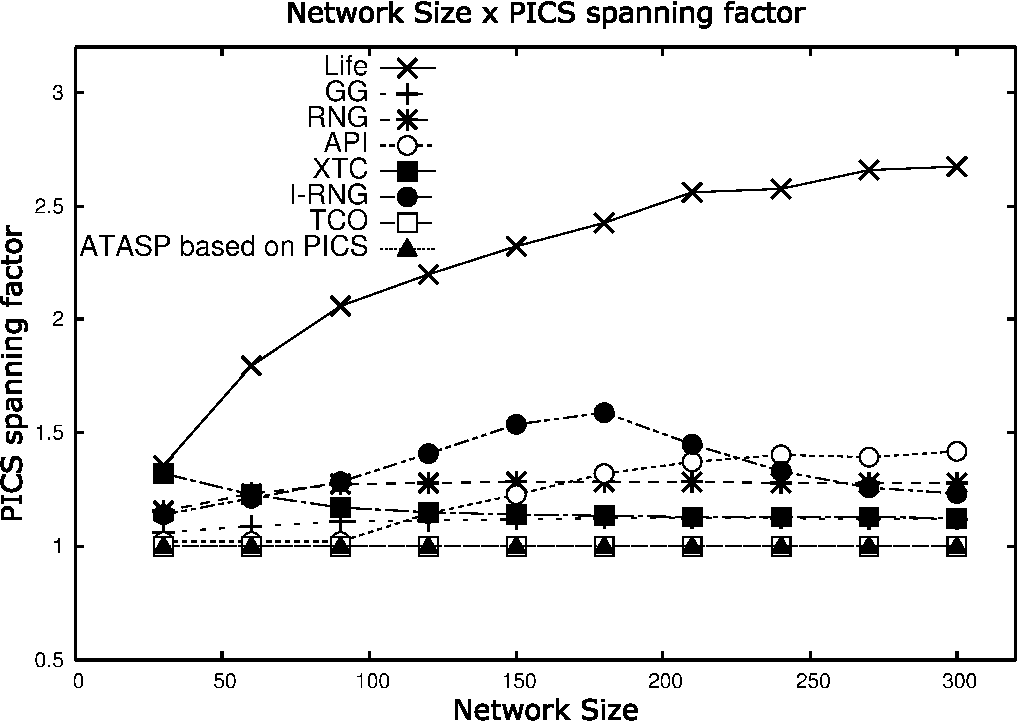
\includegraphics[scale=0.35]{sigma_average}
\caption{PICS spanning factor}
\label{fig:sigma_interference}
\end{minipage}
\hspace{0.3cm}
\begin{minipage}[b]{0.46\linewidth}
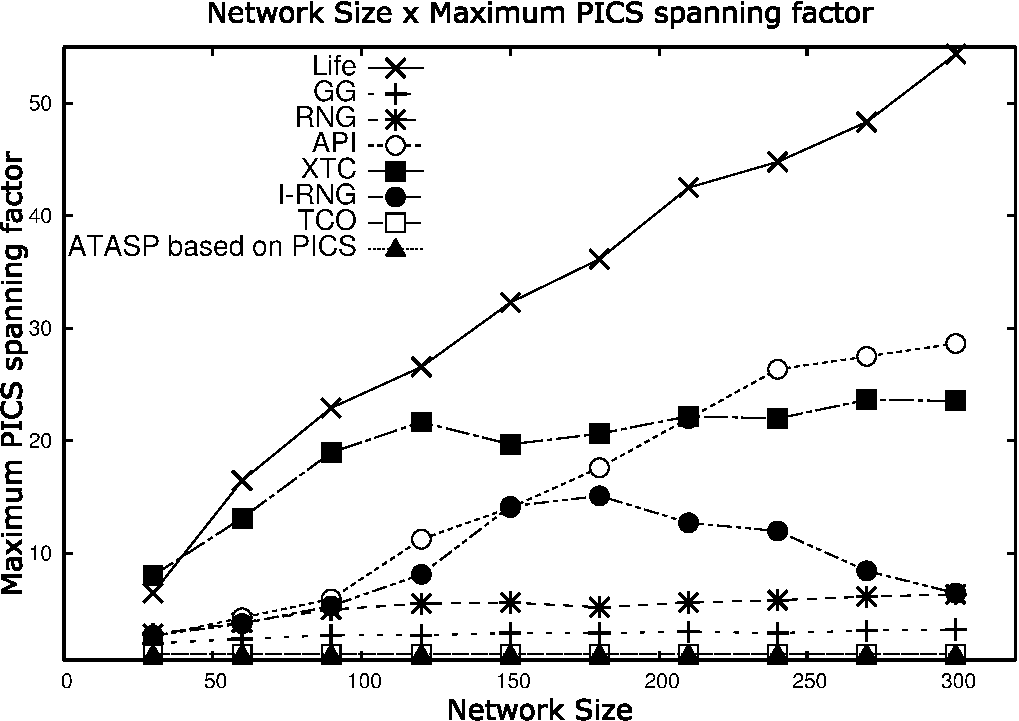
\includegraphics[scale=0.35]{sigma_max}
\caption[]{Maximum PICS spanning factor}
\label{fig:max_sigma_interference}
\end{minipage}
\end{figure}

We compared TCO against these algorithms for the following reasons. As described in Section \ref{sec-related-work}, API, \mbox{I-RNG}, \mbox{I-LMST} and LLISE are the only
localized algorithms that address interference explicitly. We did not compare TCO with I-LMST because I-RNG requires fewer message exchanges, implying a smaller overhead
(I-LMST and I-RNG were both proposed in  \cite{Li05}). 
We compared TCO with LIFE instead of LLISE because LIFE is a centralized algorithm that performs
better than LLISE (according to \cite{burkhart2004}).  
The ATASP algorithm, as proposed in \cite{blough2005}, provides topologies with optimal PIC spanning factor, i.e. $\rho$(ATASP) = 1.
In our experiments, we modified ATASP to use PICS (instead of PIC). ATASP based on PICS also has optimal PICS spanning factor, i.e. 
$\sigma$(ATASP) = 1 (it follows from the way edges are chosen in the final topology found by ATASP). 
XTC is a very simple algorithm that provides good energy spanners (on average-case graphs) \cite{Wattenhofer2004}.
We compared TCO with GG because GG presented good results in \cite{blough2005} for an interference metric similar to ours. In particular, it outperformed the algorithms CBTC \cite{Li2005} and KNeigh \cite{Santi2003}. Finally, we compared TCO with RNG because it is another classical result of computational geometry upon
which many topology control results are based.

For all algorithms, except GG and RNG, we modelled the transmissions considering the power levels of the transceiver. 
For GG and RNG we used the exact distance between nodes as these algorithms are based on geometrical properties of the network
(the definition of the resulting topology is based on distances between nodes).

Figure \ref{fig:sigma_interference} shows the mean PICS spanning factor ($\sigma$) for the topology control algorithms. 
Observe that $\sigma$ presents a constant or decay behaviour for all algorithms, except for LIFE and API. 
Observe that, in the case of TCO, $\sigma$ follows the optimum which is represented by ATASP (based on PICS) - the lines of
TCO and ATASP appear superposed.

Figure \ref{fig:max_sigma_interference} shows a comparison of the algorithms based on maximum $\sigma$, which corresponds to the worst case for each specific scenario.
Observe that maximum $\sigma$ increases quickly when compared to the average $\sigma$. 
The relative behaviour of the algorithms is similar, except for XTC, which exhibits a worse performance when maximum $\sigma$ was considered.
However, except for TCO, I-RNG (after a certain point) and ATASP, the maximum PICS spanning factor tends to increase with network size. Thus TCO and I-RNG (localized algorithms)
support better network scalability.

A special fact is that TCO presented a behaviour which is extremely close to the optimum, even with the increase in the network size. All the other algorithms exhibited
an increase in the maximum PICS spanning factor with an increase in the network size. After a certain point the maximum PICS spanning factor decreased for I-RNG (similar to what happened
in Figure \ref{fig:sigma_interference}). TCO is, therefore, the most scalable localized algorithm (according to these experiments).

Our results are consistent with the results presented in \cite{blough2005}. First, LIFE did not exhibit good performance compared to the other
algorithms. In fact, as explained in \cite{blough2005}, algorithms based on \emph{Minimum Spanning Tree} (such as LIFE) are not efficient when considering multihop interference.
Second, the PIC spanning factor increases for GG and RNG as the network density increases and GG outperforms RNG. Similar behaviour occurred to maximum $\sigma$, as can be seen
in Figure \ref{fig:max_sigma_interference} - recall that the PIC spanning factor is based on maximum values.

% ?? coloquei "metros" no paragrafo abaixo tambem

We also ran additional experiments, first with higher density, i.e., the same number of nodes but on 400m x 400m and 200m x 200m areas, 
and then with $\alpha=3$ (200m x 200m region with 300 nodes). 
In all these experiments, the behaviour of TCO was similar to the previous cases. TCO exhibited an extremely good performance, outperforming the other algorithms
and again matching the performance of ATASP (based on PICS). We do not present these results here due to lack of space.

TCO differs from GG, RNG, API, XTC and I-RNG in the fact that these protocols are based on simple triangular inequality, i.e., they consider paths up to two hops when searching for interference-efficient paths, while TCO considers (at the two-hop vicinity of nodes) general paths (with length $k$, $k \geq 2$). This might be one reason for the better performance of
TCO in relation to these algorithms.
It is important to note that TCO is not the algorithm that removed the highest number of edges from the original graph. In fact, LIFE and GG removed many more edges than TCO. 

According to our experiments and the metric we used, TCO exhibited an extremely good performance. When considering multihop interference, TCO, which is a 
distributed localized topology control algorithm (thus is based on partial knowledge of the graph), exhibited a performance equivalent to an optimal global algorithm, i.e.
based on information about the whole network. Additionally, TCO minimizes multihop interference and energy expenditure at the same time 
(i.e. it does not provide a compromise solution between these two goals).

\section{Conclusion}
\label{sec-conclusion}

This paper presented TCO as a distributed and localized topology control algorithm for optimizing interference. TCO takes into consideration
the overhearing cost and generates topologies that might have asymmetric links. As these characteristics of TCO deviate from the assumptions adopted in
many previous works on topology control, we emphasized arguments to support them. 
Further, we demonstrated that when considering overhearing, 
we achieved an algorithm that minimizes energy and is very efficient in terms of interference.

In order to compare TCO with other algorithms, we defined a new interference metric ($\sigma$).
This metric is different from previous ones because it is based on the sender-centric perspective, on the notion of interference along multihop paths and 
on the node-based approach.

The experiments were performed taking into consideration discrete power levels of transmission. The values used in the experiments were based on values
of a transceiver commonly used in real sensor networks (CC2420). We compared TCO against existing localized topology
control algorithms for interference. According to our experiments and the used metric, TCO outperformed 
all the other algorithms and, more importantly, its performance was equivalent to the performance of a centralized algorithm (optimal for the related
PIC spanning factor).

\bibliographystyle{splncs03}
\bibliography{adhocnow}
\end{document}

% ?? acertei as referencias 19 (para aparecer IEEE ao inves de ieee) e 33 (para aparecer XTC ao inves de Xtc)

?? secao 5: quarto paragrafo